% Changing book to article will make the footers match on each page,
% rather than alternate every other.
%
% Note that the article class does not have chapters.
\documentclass[letterpaper,10pt,twoside,twocolumn,openany]{book}

% Use babel or polyglossia to automatically redefine macros for terms
% Armor Class, Level, etc...
% Default output is in English; captions are located in lib/dndstring-captions.sty.
% If no captions exist for a language, English will be used.
%1. To load a language with babel:
%	\usepackage[<lang>]{babel}
%2. To load a language with polyglossia:
%	\usepackage{polyglossia}
%	\setdefaultlanguage{<lang>}
\usepackage[english]{babel}
%usepackage[italian]{babel}
% For further options (multilanguage documents, hypenations, language environments...)
% please refer to babel/polyglossia's documentation.

\usepackage[utf8]{inputenc}
\usepackage{hang}
\usepackage{lipsum}
\usepackage{listings}

%packages used for hyperlinking
\usepackage{hyperref}
\hypersetup{
	colorlinks=true,
	linkcolor=blue,
	filecolor=magenta,      
	urlcolor=cyan,
}

\usepackage{dnd}

\lstset{%
  basicstyle=\ttfamily,
  language=[LaTeX]{TeX},
}

\usepackage{eso-pic}
\newcommand\BackgroundPic{%
	\put(0,0){%
		\parbox[b][\paperheight]{\paperwidth}{%
			\vfill
			\centering
			
\includegraphics[width=\paperwidth,height=\paperheight,%
			keepaspectratio]{img/paper.jpg}%
			\vfill
}}}

\title{Sir Dexter Fahs Schweitzer Whitemace, Wielder of the Chalice of Light} 	
\author{Antonius Torode}
\date{Latest update: \today}


% Start document
\begin{document}

%\AddToShipoutPicture*{\BackgroundPic}
\maketitle
%\tableofcontents

% Your content goes here
\onecolumn
% Comment this out if you're using the article class.
\section{Backstory}

\begin{quote}
	``It all started a few centuries ago. The way the story goes is we were a peaceful people with no true purpose. We were advancing our technology and knowledge of dark magics and things were getting out of hand. We rejected any divine propaganda that was making it our way, as we were above the need for such superstitions. However, if we had stayed the path we were on we would have likely destroyed ourselves. We lived in large city called Proficiscentur on an island off the Northwest coast of Castiana about 800 km out from the mainland. We stuck to our roots in science until the day came when we saw the truth. 

	Like a thief in the night, the followers of the Celestials came with raging machines. They were normally a simple people, keeping to their religion and tending to their farmlands. But this day, the Celestials showed their true power and divine nature. It's one thing for a people to spend their lives rejecting false gods, but when the true power of real gods knock, you can't choose to keep the door closed. They infiltrated our city and burned every last being that stood in their way. They utterly destroyed Proficiscentur (the city of the advanced). Their power was unlike anything you could imagine. They came in with staffs of magic missile and armor of pure energy. It was said that just one of their ships was strong enough to take out all that we had. There was no doubt that there was a true power from deities with these people.
	
	Those in the outskirts of the island realized they could not defy these beings and accepted defeat. Through time, they rebuilt the great city, this time named Renascitur (the city of the reborn). Over the first hundred years our people struggled as there were small terrorist groups fightings against the change. Small resistance forces that tried to defy the Celestials. All perished. Those of us that were left finally understood that the Celestials were saving us from a fate that we were dooming ourselves to. We were ignoring the true power of the Celestials that were right at our doorstep and trying to advance our lives to a salvation on our own. With no purpose before, we now had the Celestials to show us the true light and path to enlightenment. With the hope and promises in the Book of Celestas, we now had a purpose to exist. There was no longer a desire for advancement, because if technology was needed, the Celestials would provide, as long as we followed their ways.
	
	That's at least how my great granddaddy puts the story. All I know is I've seen miracles of the Celestials with my own eyes. Their power is infinite and their promises cannot be ignored. After being born and raised into the faith, I've never had a reason to doubt what they have showed me.''
\end{quote}

At this point Dex begins chugging his ale. Looks around at the other bar folk waiting for him to answer their question about where he got his war hammer. Dex blinks and looks around and the last drops of fizz fall down the side of the mug.

\begin{quote}
	``The war hammer was a gift, from one of the Priors who guide us. It is said to have been plucked from a place called Nidavellir deep within the Pluvian realm of Statu. It was forged to contain the pure essence of energy. When it burns with its sacred flames, I know the Celestials are with me in what I am doing. When the flames go out, I know I need to seek guidance. It is a great reminder that my strength comes from they. Hallowed are the Celestials.''
\end{quote}

He raises his empty mug in one hand, and the war hammer in another. The flames of the war hammer illuminate and irradiate energy all throughout the tavern. Magically, the ale levels in his cup seem to refill. In amazement, the folk of the pub seem dazzled at the power of the war hammer.

\begin{quote}
	``Don't think this hammer has any real power my friends. The real power within it is held with the Celestials. They are the only true gods with a real promise of salvation and enlightenment. If you follow them and their ways, you will never see a dull moment.''
\end{quote}

A shadowy figure in a dark cloak sitting in the corner of the tavern stands up and walks over. ``How do your Celestials spread their teachings?'' Dex looks up at him after lowering his hands and war hammer. ``What is your name mystery man?'' The shadowy figure pulls his hood over his head and looks up. ``I am Dastan, I wish to know of the Celestials.'' Dex reaches deep into his bag.

\begin{quote}
	``The Book of Celestas teachings the ways to enlightenment, I have traveled far on this sacred journey of mine and spread the word throughout the land. This copy is my last book to hand out before I need to make others. You may have it. Follow it's ways and you will be rewarded. The day of the lamb is near, where all will know the true power and truth of the Celestials. Et terra rus ad sidera tollere vultus. Ex uno disce omnes.''
\end{quote}

After muttering the words straight from the book of Celestas, he hands another copy of the book and his newly filled beer to Dastan and hops out of his chair to leave the bar. His presence seems almost with utter important and Dastan says nothing in return. Dastan takes the book and retreats to his corner, placing the cloak covering back over his head. Dex leaves the tavern wondering where to head next, knowing he must seek to spread the influence of the Celestials throughout the world.

\section{Class Features}

\subsection{Ability Scores (level 5)}
\stats[STR = \stat{16},DEX = \stat{7},CON = \stat{14},INT = \stat{14},WIS = \stat{16},CHA = \stat{12}]

\subsection{Traits}
\begin{description}
	\item[Ability score increase:] Your ability scores each	increase by 1.
	\item[Age:] 42
	\item[Alignment:] Lawful Neutral 
	\item[Size:] 5'9"
	\item[Speed:] 30 ft.
	\item[Languages:] Common, 
\end{description}

\subsection{Cleric Hit Points}

\begin{description}[font=\normalfont\textbf,noitemsep,topsep=1ex,leftmargin=1em]
	\item[Hit Dice:] 1d8 per cleric level
	\item[Hit Points at First Level:] 8 + constitution modifier
	\item[Hit Points at Higher levels:] 1d8 + constitution modifier per cleric level after first
\end{description}

\subsection{Proficiencies}

\begin{description}[font=\normalfont\textbf,noitemsep,topsep=1ex,leftmargin=1em]
	\item[Armor:] Light armor, medium armor, shields
	\item[Weapons:] All simple weapons
	\item[Tools:] None
	\item[Other:] Driving Warthags
\end{description}

\begin{description}[font=\normalfont\textbf,noitemsep,topsep=1ex,leftmargin=1em]
	\item[Saving Throws:] Wisdom, Charisma
	\item[Skills:] Choose two from History, lnsight, Medicine, Persuasion, and Religion
\end{description}

\subsection{Equipment}

\begin{description}
	\item (a) a mace or (b) a warhammer (if proficient)
	\item (a) scale mail, (b) leather armor, or (c) chain mail (if proficient)
	\item (a) a light crossbow and 20 bolts or (b) any simple weapon
	\item (a) a priest's pack or (b) an explorer's pack
	\item A shield and a holy symbol
\end{description}

\subsection{Spell Casting}

\begin{center}
	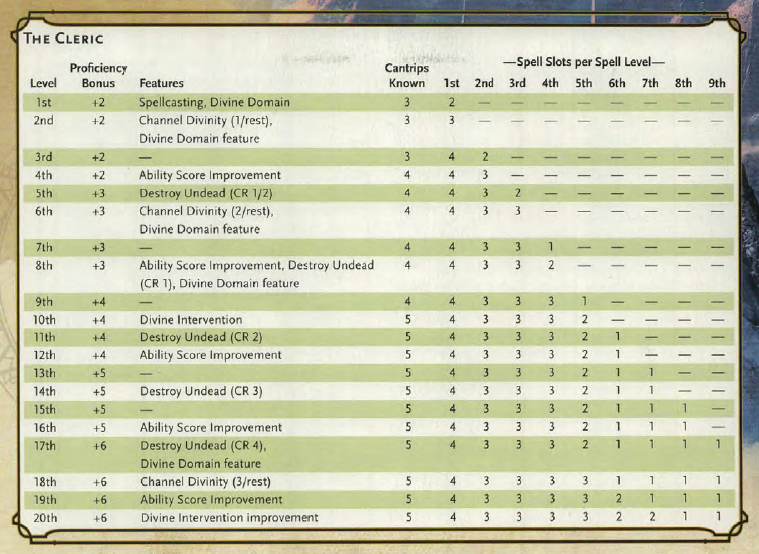
\includegraphics[width=\linewidth]{img/ClericTable.png}
\end{center}

\subsubsection{Cantrips}

At 1st level, you know three cantrips of your choice from the cleric spell list. Vou learn additional cleric cantrips of your choice at higher levels, as shown in the cantrips Known column of the Cleric table.

\subsubsection{Preparing and Casting Spells}

The Cleric table shows how many spell slots you have to cast your spells of 1st level and higher. To cast one of these spells, you must expend a slot of the spell's level or higher. Vou regain all expended spell slots when you finish a long rest.

You prepare the list of cleric spells that are available for you to cast, choosing from the cleric spell list. When you do 50, choose a number of cleric spells equal to your Wisdom modifier + your cleric level (minimum of one spell). The spells must be of a level for which you have spell slots.

For example, if you are a 3rd-Ievel c1eric, you have four 1st-level and two 2nd-level spell slots. With a Wisdom of 16, your list of prepared spells can include six spells of 1st or 2nd level, in any combination. if you prepare the 1st-level spell cure wounds, you can cast it using a 1st-level or 2nd-level slot. Casting the spell doesn't remove it from your list of prepared spells.

You can change your list of prepared spells when you finish a long rest. Preparing a new list of cleric spells requires time spent in prayer and meditation: at least 1 minute per spell level for each spell on your list.

\subsubsection{Ritual Casting}

You can cast a cleric spell as a ritual if that spell has the ritual tag and you have the spell prepared.

\subsection{Divine Domain}

Choose one domain related to your deity: Knowledge, Life, Light, Nature, Tempest, Trickery, or War. Each domain is detailed at the end of the class description, and each one provides examples of gods associated with it. Your choice grants you domain spells and other features when you choose it at 1st level. It also grants you additional ways to use Channel Divinity when you gain that feature at 2nd level, and additional benefits at 6th, 8th, and 17th levels.

\subsubsection{Domain Spells}

Each domain has a list of spells-its domain spells that you gain at the cleric levels noted in the domain description. Once you gain a domain spell, you always have it prepared, and it doesn't count against the number of spells you can prepare each day If you have a domain spell that doesn't appear on the cleric spell list, the spell is nonetheless a cleric spell for YOU.

\subsection{Channel Divinity}

At 2nd level, you gain the ability to channel divine energy directly from your deity, using that energy to fuel magical effects. You start with two such effects: Turn Undead and an effect determined by your domain. Some domains grant you additional effects as you advance in levels, as noted in the domain description. When you use your Channel Divinity. you choose which effect to create. Vou must then finish a short or long rest to use your Channel Divinity again. Some Channel Divinity effects require saving throws. When you use such an effect from this class, the DC equals your c1eric spell save DC. Beginning at 6th level, you can use your Channel Divinity twice between rests, and beginning at 18th level, you can use it three times between rests. When you finish a short or long rest, you regain your expended uses.

\subsubsection{Channel Divinity: Turn Undead}

As an action, you present your holy symbol and speak a prayer censuring the undead. Each undead that can see or hear you within 30 feet of you must make a Wisdom saving throw. If the creature fails its saving throw, it is turned for 1 minute or until it takes any damage. A turned creature must spend its turns trying to move as far away from you as it can, and it can't willingly move to a space within 30 feet of you. lt also can't take reactions. For its action, it can use only the Dash action or try to escape from an effect that prevents it from moving. If there's nowhere to move, the creature can use the Dodge action.

\subsection{Destroy Undead}

Starting at 5th level, when an undead fails its saving throw against your Turn Undead feature, the creature is instantly destroyed if its challenge rating is at or below a certain threshold, as shown in the Destroy Undead table.

\begin{dndtable}
	\textbf{Cleric level}  & \textbf{Destroys Undead of CR...} \\
	5th level  & $\frac{1}{2}$ or lower \\
	8th level  & 1 or lower \\
	11th level  & 2 or lower
\end{dndtable}

\subsection{Knowledge Domain}

\begin{dndtable}
	\textbf{Cleric level}  & \textbf{spells} \\
	1st & Command, Identify \\
	3rd & Augury, Suggestion \\
	5th & Nondetection, Speak with Dead \\
	7th & Arcane Eye, Confusion \\
	9th & Legend Lore, Scrying
\end{dndtable}

\subsubsection{Blessing of Knowledge}

At 1st level, you learn two languages of your choice. You also become proficient in your choice of two of the following skills: Arcana, History, Nature, or Religion. Your proficiency bonus is doubled for any ability check you make that uses either of those skills.

\subsubsection{Channel Divinity: Knowledge of the Ages}

Starting at 2nd level, you can use your Channel Divinity to tap into a divine well of knowledge. As an action, you choose one skill or tool. For 10 minutes, you have proficiency with the chosen skill or tool.

\subsubsection{Channel Divinity: Read Thoughts}

At 6th level, you can use your Channel Divinity to read a creature's thoughts. You can then use your access to the creature's mind to command it.

As an action, choose one creature that you can see within 60 feet of you. That creature must make a Wisdom saving throw. If the creature succeeds on the saving throw, you can't use this feature on it again until you finish a long rest.

If the creature fails its save, you can read its surface thoughts (those foremost in its mind, reflecting its current emotions and what it ie actively thinking about) when it is within 60 feet of you. This effect lasts for 1 minute.

During that time, you can use your action to end this effect and cast the Suggestion spell on the creature without expending a spell slot. The target automatically fails its saving throw against the spell.

\subsection{Spell casting Ability}

\begin{description}
	\item[Spell save DC:] 8 + proficiency bonus + wisdom modifier 
	\item[Spell attack modifier:] proficiency bonus + wisdom modifier
\end{description}

\section{Background: Folk Hero}

\begin{description}[font=\normalfont\textbf,noitemsep,topsep=1ex,leftmargin=1em]
	\item[Ski1l Proficiencies:] Animal Handling, Survival
	\item[Tool Proficiencies:] One type of artisan's tools,	vehicles (land)
	\item[Equipment:] A set of artisan's tools (one of your choice), a shovel, an iran pot, a set of common clothes, and a belt pouch containing 10 gp
\end{description}

\subsubsection{Rustic Hospitality}

Since you come from the ranks of the common folk, you fit in among them with ease. Vou can find a place to hide, rest, or recuperate among other commoners, unless you have shown yourself to be a danger to them. They will shield you from the law or anyone else searching for you, though they will not risk their lives for YOU.

\subsection{Chalice of Light}

The Chalice of Light is known in Legend to be a holy war hammer imbued directly with the presence of a divine spirit. It is believed that Apollo had a follower so loyal and faithful that Apollo sent an angel to reside within this particular war hammer and protect the wielder during his dangerous missionary journeys. The hammer was originally forged by a dwarven clan which dedicated themselves to Apollo. Per legend, a high priest of Apollo took it upon himself to set forth into the most dangerous lands to preach that of Apollo. Among his second journey, he found himself being ambushed and sent to his death in a place called The Undercity. In a fervent prayer, his war hammer became light to the tough, and changed it's appearance to hold an everlasting flame that burned alongside his faith and gave the high priest the ability to break free from his bonds and purge The Undercity of the sins that corrupted it and the surrounding lands. The flame of the burning hammer is said to have ceased when the wielder died of old age. It is believed that if the hammer is found, it is already forged to hold the essence of an angel and can provide uncanny abilities to a man of great faith.

\begin{center}
	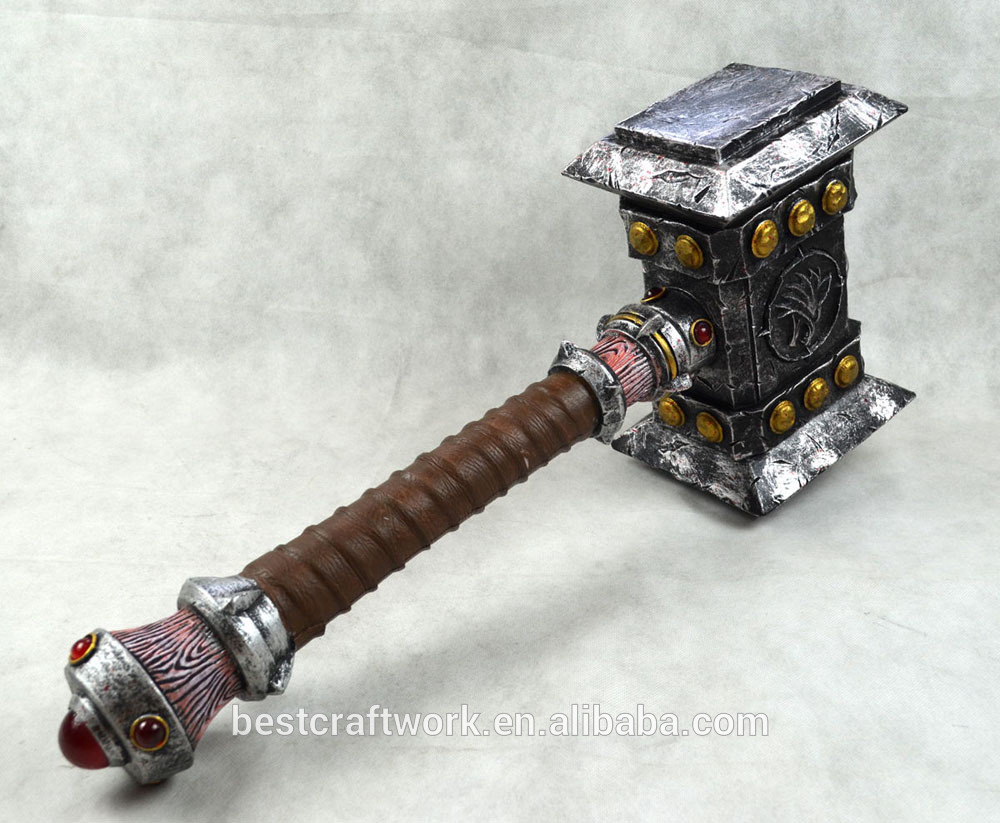
\includegraphics[width=0.41\linewidth]{img/Wow-Hammer.jpg} 	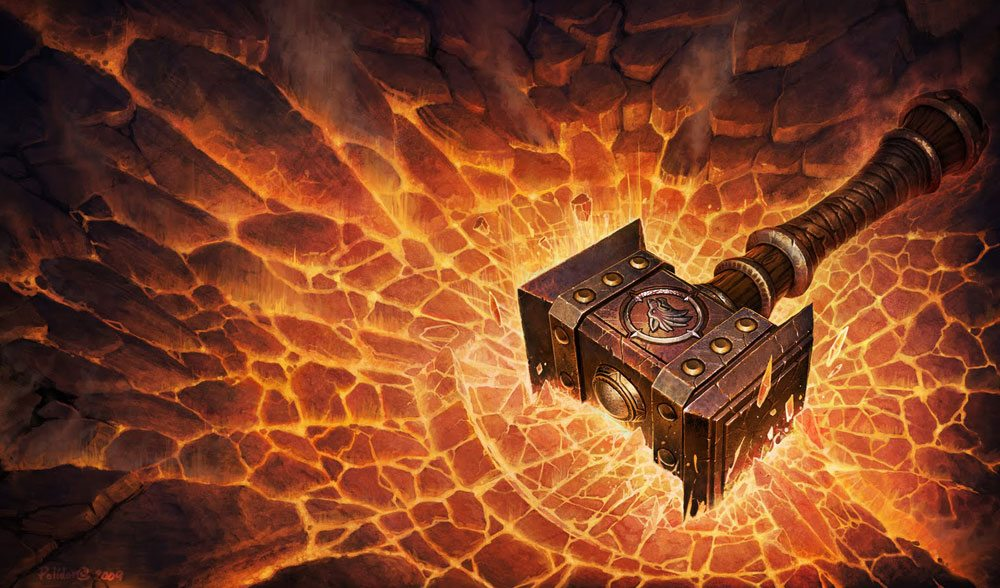
\includegraphics[width=0.57\linewidth]{img/shatteredhand.jpg}
\end{center}

\subsubsection{Potential}

The Chalice of Light weapon wants to be wielded by a religious character. 

\begin{commentbox}{Chalice of Light\footnote{Weapon (warhammer), artifact (requires attunement by a cleric)}}	
	If no angel or spirit from a deity is with this weapon, it is a simple warhammer that only does 1d8 bludgeoning damage.
	
	You gain a +3 bonus to attack and damage rolls made with this magic weapon. When you hit an enemy you will deal 1d6 fire damage and 1d6 radiant damage. The damage will change to d10's if the target rejects the clerics deity (they must know of them though).
	
	When you take damage while wielding the Chalice of Light, you can heal one target within 50 yards for a single roll of the dice closes to the wielders level (round up).
	
	While a cleric wields The Chalice of Light in combat it will look like the cleric is burning with a holy flame. Anyone who rejects the clerics deity that attacks the wielder will take 1d6 fire damage and 1d6 radiant damage. When the wielder rolls a 20 against someone who rejects their deity, the wielder must make a d100 roll. If the roll is less than half the wielders lvl then the attacker will burn in holy flame and turn to ash immediately.
	
	If a cleric of an evil alignment tries to attune to The Chalice of Light they have to make a d20 roll. At a 18 or below The Chalice of Light will reject you and deal 3d10 fire damage and 2d10 radiant damage. At a 19 or 20 you over power the will of the weapon and make it yours.
	
	With a successful roll to overcome the will of The Chalice of Light while having an evil alignment will make The Chalice of Light's appearance will start to dull and become darker until it becomes fully corrupt. It will regain its former glory when its attuned to a cleric of a non evil alignment.
	
	Proficiency with a warhammer allows you to add your proficiency bonus to the attack roll for any attack you make with it.
	
	If the wielder of Chalice of Light dies (by failing three death saves) then the angel within the hammer can leave the weapon and resurrect the player to full. The weapon after this point becomes useless.
\end{commentbox}

\subsection{Quotes}

% End document
\end{document}
